\chapter{Introducción a la Teoría Descriptiva de Conjuntos}

La Teoría Descriptiva de Conjuntos (TDC a partir de ahora) tiene como un objetivo clasificar enunciados o fórmulas según su complejidad, concepto que luego formalizaremos. Por ejemplo, si consideramos sobre las funciones del intervalo $[0,1]$ en $\mathbb{R}$ la propiedad de ``ser continua'':
\begin{equation*}
    \forall x\in [0,1]\ \forall \veps > 0\ \exists \delta>0 : \forall x_0\ |x-x_0|<\delta \Longrightarrow |f(x)-f(x_0)|<\veps
\end{equation*}

Como sabemos que toda función continua en $[0,1]$ es uniformemente continua y que toda función uniformemente continua es continua, podemos reescribir esta propiedad de una forma ``menos compleja'', eliminando en $\veps$ la dependencia de $x$
\begin{equation*}
    \forall \veps > 0\ \exists \delta>0 : \forall x_0\ |x-x_0|<\delta \Longrightarrow |f(x)-f(x_0)|<\veps
\end{equation*}
y obteniendo así una fórmula más corta, algo que nos interesará, puesto que intentaremos buscar las fórmulas más cortas (en función de las variables y cuantificadores que aparecen en ellas) que nos definan ciertas propiedades.

\section{Construcción de fórmulas}
Sin olvidar que la teoría sobre la que trabajamos (la de Zermelo-Fraenkel) es en particular un lenguaje de primer orden, recordamos que nuestras fórmulas van a estar formadas por, fijado un conjunto $X$ que contendrá los elementos a los que nos refiramos:
\begin{itemize}
    \item Términos, referidos a objetos.
    \item Conectores: $\lnot$, $\land$, $\lor$, $\rightarrow$, $\leftrightarrow $.
    \item Cuantificadores: $\forall $, $\exists $.
\end{itemize}
De esta forma, una fórmula para nosotros será una composición \underline{finita} de estos elementos.\\

Estaremos especialmente interesados en el hecho de que las fórmulas sean composiciones finitas de dichos elementos, así como en estudiar los cuantificadores que aparecen en las fórmulas.

\begin{ejemplo}
    Si consideramos $X = \mathbb{N}$ y en este contexto consideramos la aplicación ``sucesor'' $s:\mathbb{N}\to \mathbb{N}$, la fórmula:
    \begin{equation*}
        s\leq s(n)
    \end{equation*}
    Contiene a $n$ como variable libre, y (en general) podrá ser cierta o falsa en función de las sustituciones de $n$ realicemos (aunque en este caso hemos considerado una fórmula que ante cualquier sustitución siempre es cierta).
\end{ejemplo}

A partir de ahora, lo que nos interesará es dada una fórmula $P$ en la que hay una variable libre y trabajando sobre un conjunto $X$, podremos siempre considerar por el axioma de composición el conjunto formado por aquellos elementos de $X$ para los cuales la fórmula $P$ sea cierta:
\begin{equation*}
    X_P = \{x\in X \mid P(x) \}
\end{equation*}
Sin embargo, el recíproco de esta afirmación (que para cada cojunto siempre podemos encontrar una fórmula que cumplan exclusivamente los elementos del conjunto) no será generalmente cierta. Por ejemplo, si consideramos $X$ un conjunto finito, como $\cc{P}(X)$ es finito, siempre podremos hacerlo; pero en un caso general con $X$ cualquier conjunto (posiblemente no numerable), podemos pensar en que la cantidad de fórmulas que podemos construir es un conjunto numberable, por lo que no llegaremos a abarcar todas las posibilidades\footnote{Es mucho más complejo que esto, este argumento no es suficiente para demostrarlo.}.

\begin{ejemplo}
    Como primeros ejemplos de conjuntos a destacar, fijado un conjunto $X$, consideramos una cantidad numerable de subconjuntos de $X$: $\{X_n\}_{n\in \mathbb{N}}$ con $X_n\subseteq X$ para todo $n\in \mathbb{N}$.
    \begin{itemize}
        \item Si pensamos en la intersección de todos estos conjuntos:
            \begin{equation*}
                \bigcap_{n\in \mathbb{N}} X_n
            \end{equation*}
            Podemos tratar de buscar una fórmula que defina única y exclusivamente a todos los elementos de este conjunto, como por ejemplo:
            \begin{equation*}
                \forall n(n\in \mathbb{N} \Longrightarrow x\in X_n)
            \end{equation*}
        \item Si ahora consideramos la unión de todos ellos: 
            \begin{equation*}
                \bigcup_{n\in \mathbb{N}}X_n
            \end{equation*}
            Y tratamos de buscar una fórmula que lo defina, llegamos a:
            \begin{equation*}
                \exists n(n\in \mathbb{N} \land x\in X_n)
            \end{equation*}
    \end{itemize}
\end{ejemplo}

A partir de este primer ejemplo y viendo la relación existente entre los cuantificadores $\forall $ y $\exists $ con las operaciones $\cap$ y $\cup$, buscamos ahora cómo podemos expresar ciertas fórmulas sobre algún espacio $X$ previamente fijado en forma de conjuntos, proceso que ilustraremos con los siguientes ejemplos.

\begin{ejemplo}
    En cada caso, consideraremos un conjunto $X$ distinto.
    \begin{itemize}
        \item En el espacio de las sucesiones de números reales: $X = \mathbb{R}^\mathbb{N} = \{x:\mathbb{N}\to \mathbb{R}\}$

            Pensamos en la propiedad de que una sucesión sea ``casi nula'', que intuitivamente podemos definir como que una sucesión tenga una cantidad infinita de términos nulos. De manera formal, podemos escribir que existe un término a partir del cual todos los términos de la sucesión son cero:
            \begin{equation*}
                \exists n\in \mathbb{N}\ \forall m\geq n\ x(m) = 0
            \end{equation*}
            Que podemos escribir de forma más rigurosa como (entendiendo que donde pone $m\geq n$ deberíamos escribir $m\geq n \land m\in \mathbb{N}$):
            \begin{equation*}
                \exists n(n\in \mathbb{N} \land \forall m(m\geq n \Longrightarrow x(m) = 0))
            \end{equation*}
            Donde observamos que en esta la variable $x$ aparece libre, por lo que podemos tratar de buscar un conjunto que contenga todos aquellos elementos que cumplan la fórmula para cierto $x$ y ninguno más, conjunto al que denotaremos por $C_{00}$.

            Para hayar este conjunto, lo que haremos será en primer lugar considerar los términos que aparecen en la fórmula y en segundo lugar, tratar de relacionarlos con los conectores y cuantificadores que aparecen. Para ello, los términos que aparecen en la fórmula son:
            \begin{equation*}
                n\in \mathbb{N} \qquad m\geq n \qquad x(m) = 0
            \end{equation*}
            Y para construir el conjunto que venga definido por la fórmula, lo que haremos será ir poco a poco de dentro hacia afuera, considerando primero el conjunto que cumpla:
            \begin{equation*}
                x(m) = 0
            \end{equation*}
            De esta forma, fijado $m$, definimos:
            \begin{equation*}
                X_m = \{x\in \mathbb{R}^\mathbb{N} : x(m) = 0\}
            \end{equation*}
            Ahora, buscamos el conjunto que venga definido por la fórmula:
            \begin{equation*}
                \forall m(m\geq n\Longrightarrow x(m) = 0)
            \end{equation*}
            Que podemos reescribir como:
            \begin{equation*}
                \forall m(m\geq n\Longrightarrow x\in X_m)
            \end{equation*}
            Observando el $\forall $, podemos pensar en reescribir este conjunto como en una intersección de conjuntos:
            \begin{equation*}
                \bigcap_{m\geq n}X_m
            \end{equation*}
            Finalmente, la fórmula entera:
            \begin{equation*}
                \exists n(n\in \mathbb{N} \land \forall m(m\geq n \Longrightarrow x(m) = 0))
            \end{equation*}
            La podemos reescribir como:
            \begin{equation*}
                \exists n\left(n\in \mathbb{N} \land x\in \bigcap_{m\geq n} X_m\right)
            \end{equation*}
            Que podemos expresar ahora como la unión de ciertos conjunto.
            \begin{equation*}
                \bigcup_{n\in \mathbb{N}}\bigcap_{m\geq n} X_m
            \end{equation*}
            Obteniendo así nuestro conjunto $C_{00}$:
            \begin{equation*}
                C_{00} = \bigcup_{n\in \mathbb{N}}\bigcap_{m\geq n} X_m
            \end{equation*}
        \item Sobre el mismo espacio $X= \mathbb{R}^\mathbb{N}$ podemos ahora considerar la propiedad de ``ser convergente a 0'', propiedad definida por:
            \begin{equation}\label{eq:conv_0}
                \forall \veps > 0\ \exists m\in \mathbb{N}\ \forall n\geq m \Longrightarrow |x(m)| < \veps
            \end{equation}
            Y que de forma rigurosa puede escribirse como (entendiendo que donde pone $n\geq m$ deberíamos escribir $n\geq m \land n\in \mathbb{N}$ y que donde pone $\veps > 0$ deberíamos poner $\veps \in \mathbb{R}^+$):
            \begin{equation*}
                \forall \veps(\veps > 0 \Longrightarrow \exists m(m\in \mathbb{N} \land \forall n(n\geq m \Longrightarrow |x(m)|<\veps)))
            \end{equation*}
            Fórmula a partir de la cual podemos extrar un conjunto de igual forma que hicimos anteriormente, identificando que los términos son:
            \begin{equation*}
                \veps > 0 \qquad m\in \mathbb{N} \qquad n\geq m \qquad |x(m)|<\veps
            \end{equation*}
            Y construyendo la fórmula de dentro hacia afuera. Para ello, en primer lugar, fijados $m$ y $\veps$ definimos el conjunto:
            \begin{equation*}
                X_{n,\veps} = \{x\in \mathbb{R}^\mathbb{N} : |x(n)|<\veps\}
            \end{equation*}
            Y posteriormente escribiendo las sucesivas fórmulas como uniones e intersecciones, llegando a:
            \begin{equation*}
                \bigcap_{\veps > 0} \bigcup_{m\in \mathbb{N}} \bigcap_{n\geq m} X_{n,\veps}
            \end{equation*}
            Sin embargo, hay una diferencia ahora entre la fórmula obtenida anteriormente y esta; resulta que en esta fórmula estamos considerando una intersección no numerable de elementos, al considerar la intersección de todos aquellos elementos de $\mathbb{R}^+$, un hecho que nos va a dificultar luego algo en lo que estamos interesados\footnote{Que es poder definir una sigma álgebra que contenga uniones e intersecciones numerables de ciertos conjuntos.}.

            A pesar de ello, la solución en este caso es bien sencilla. Resulta que la definición de convergencia a 0 cuya definición escribimos en~(\ref{eq:conv_0}) puede caracterizarse en función de una sucesión convergente a cero, pudiendo cambiar la fórmula que describe la propiedad de ``ser convergente a cero'' por la fórmula:
            \begin{equation*}
                \forall k\in \mathbb{N}\ \exists m\in \mathbb{N}\ \forall n\geq m \Longrightarrow |x(m)| < \dfrac{1}{k}
            \end{equation*}
            Si ahora realizamos nuevamente el proceso anterior de reescribir a qué conjunto llegamos, obtenemos ahora sí un conjunto dado por intersecciones y uniones numerables de ciertos conjuntos:
            \begin{equation*}
                \bigcap_{k\in \mathbb{N}} \bigcup_{m\in \mathbb{N}} \bigcap_{n\geq m} X_{n,\frac{1}{k}}
            \end{equation*}
        \item Si ahora consideramos $X = \{f:\mathbb{R}\to\mathbb{R} : f \text{\ continua}\}$ y fijado $L\in \mathbb{R}^+$, pensamos en la propiedad de $\lim\limits_{x\to\infty}f(x) = L$, definida por:
            \begin{equation*}
                \forall \veps > 0\ \exists M>0\ \forall x>M\ |f(x)-L|<\veps
            \end{equation*}
            Se nos plantea el problema anterior de que obtendríamos uniones o intersecciones no numerables de conjuntos. Sin embargo, vemos que es fácil reemplazar $\veps$ y $M$ para que esto no suceda, obteniendo una expresión equivalente:
            \begin{equation*}
                \forall k\in \mathbb{N}\ \exists M\in \mathbb{N}\ \forall x>M\ |f(x)-L|<\dfrac{1}{k}
            \end{equation*}
            Sin embargo, seguimos teniendo el problema de que $x\in \mathbb{R}$, que pensamos en cómo solucionar. Como estamos considerando funciones continuas de $\mathbb{R}$ en $\mathbb{R}$ y $\mathbb{Q}\subseteq \mathbb{R}$ es denso y numerable, podemos considerar $x\in \mathbb{Q}$ y reescribir la propiedad de forma equivalente como:
            \begin{equation*}
                \forall k\in \mathbb{N}\ \exists M\in \mathbb{N}\ \forall x\in \mathbb{Q}, x>M\ |f(x)-L|<\dfrac{1}{k}
            \end{equation*}
            Así, obtenemos una fórmula:
            \begin{equation*}
                \forall k\left(k\in \mathbb{N}\Longrightarrow \exists M\left(M\in \mathbb{N}\land \forall x\left(x\in Q\land x>M \Longrightarrow |f(x)-L|<\dfrac{1}{k}\right)\right)\right)
            \end{equation*}
            Fijado $x$ y $k$, definimos el conjunto:
            \begin{equation*}
                X_{x,k} = \left\{f\in C(\mathbb{R}) : |f(x)-L|<\dfrac{1}{k}\right\}
            \end{equation*}
            Y la fórmula nos da el conjunto:
            \begin{equation*}
                \bigcap_{k\in \mathbb{N}} \bigcup_{M\in \mathbb{N}} \bigcap_{\substack{x>M\\x\in \mathbb{Q}}} X_{x,k}
            \end{equation*}
        \item Finalmente, si ahora consideramos el mismo espacio $X$ y la pensamos en la propiedad de que una función tenga límite en infinito:
            \begin{equation*}
                \forall L\in \mathbb{R}\ \forall \veps > 0\ \exists M>0\ \forall x>M\ |f(x)-L|<\veps
            \end{equation*}
            Sabemos que podemos sustituir $\veps$, $M$ y $x$ para obtener intersecciones y uniones numerables, pero ¿cómo podemos ahora hacer esto con $L$? Pues bien, podemos usar un resultado bien conocido, y es que $\mathbb{R}$ es completo, por lo que cualquier sucesión de Cauchy es convergente y viceversa, con lo que podemos reescribir esta fórmula en una equivalente de la forma:
            \begin{equation*}
                \forall k\in \mathbb{N}\ \exists M\in \mathbb{N}\ \forall x,y\in \mathbb{Q}, x,y>M\ |f(x)-f(y)|<\veps
            \end{equation*}
    \end{itemize}
\end{ejemplo}~\\
\noindent
Con esta gran cantidad de ejemplos hemos visto cómo podemos obtener conjuntos a partir de fórmulas, así como tratar de buscar siempre una cantidad numerable de intersecciones y uniones, que generalmente obtendremos usando teoremas fundamentales del espacio en el que trabajemos.\\

En resumen, fijado un conjunto $X$, nos interesará dar propiedades mediante fórmulas, a partir de las cuales construir conjuntos mediante intersecciones y uniones (preferiblamente numerables) de conjuntos, las cuales vendrán dadas por los cuantificadores que hemos usado en la fórmula para describir una propiedad específica. De esta forma, dada una cierta propiedad y considerando una cierta topología $\cc{T}$ sobre el espacio $X$, los conjuntos que obtengamos podrán ser:
\begin{itemize}
    \item Abiertos.
    \item Cerrados.
    \item Intersecciones numerables de abiertos.
    \item Uniones arbitrarias de cerrados.
    \item Uniones numerables de intersecciones numerables de abiertos.
    \item Intersecciones numerables de uniones numerables de cerrados.
    \item \ldots
\end{itemize}
De esta forma, llegaremos luego a considerar una $\sigma-$álgebra de Borel, que será donde podamos trabajar.\\

Finalmente nos preguntamos si toda fórmula puede reducirse a unos cuantificadores numerables, pregunta cuya respuesta será que no\footnote{Se verá un leve razonamiento de por qué.}, y esta respuesta nos hará interesarnos por una noción más general de los cardinales de los conjuntos.

\section{Conjunto de Cantor}
\begin{definicion}[Conjunto de Cantor]
    Definimos el conjunto de Cantor como el conjunto de las sucesiones de $\{0,1\}$:
    \begin{equation*}
        2^{\mathbb{N}} = \{f:\mathbb{N}\to \{0,1\}\}
    \end{equation*}
\end{definicion}
\noindent
Las sucesiones de números de $\{{0,1}\}$ podemos entenderlas de forma gráfica como cada una de las elecciones (arriba o abajo) en las bifurcaciones del siguiente dibujo:
\begin{figure}[H]
    \centering
    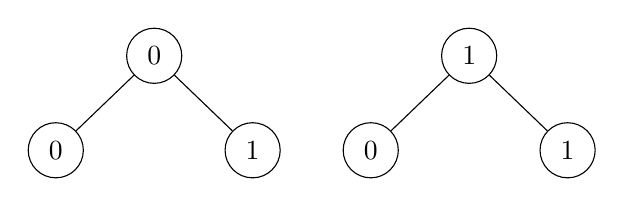
\begin{tikzpicture}[level distance=1.2cm, sibling distance=2.5cm,
      every node/.style = {circle, draw, minimum size=7mm},
      level 1/.style={sibling distance=2.5cm},
      level 2/.style={sibling distance=1.5cm}
    ]

    % Primer árbol
    \node {0}
        child {node {0}}
        child {node {1}};

    % Segundo árbol
    \begin{scope}[xshift=4cm]
    \node {1}
        child {node {0}}
        child {node {1}};
    \end{scope}

    \end{tikzpicture}
\end{figure}

\begin{notacion}
    Nos interesará también considerar una sucesión finita de elementos de $\{0,1\}$: 
    \begin{equation*}
        2^{<\mathbb{N}} = \bigcup_{n\in \mathbb{N}} \{f:\{0,1,\ldots,n\} \to \{0,1\}\}
    \end{equation*}
\end{notacion}

\noindent
Lo que nos interesará será comparar qué tan cercanas están los elementos del conjunto de Cantor entre sí de una forma intuitiva.
\begin{ejemplo}
    Por ejemplo, ante las sucesiones:
    \begin{align*}
        &(0, 1, 0, 1, 0, \ldots) \\
        &(0, 1, 1, 0, 0, \ldots) \\
        &(0, 1, 0, 1, 1, \ldots)
    \end{align*}
    Nos interesará decir que la tercera sucesión es la que más se parece a la primera. Una analogía es comparar lo que estamos haciendo con los números irracionales, ya que el conjnto de los números irracionales, $\mathbb{R}\setminus\mathbb{Q}$, podemos verlo como un entero seguido de una sucesión de naturales del conjunto $\{0,1,\ldots,9\}$:
    \begin{equation*}
        x\in \mathbb{R}\setminus\mathbb{Q}, \quad x = a'n_1 n_2 n_3 \ldots \qquad a\in \mathbb{Z}, n_1,n_2,n_3, \ldots \in \{0,1,\ldots, 9\}
    \end{equation*}
    Ante los siguientes números irracionales:
    \begin{align*}
        &3.141529\ldots \\
        &3.141578\ldots \\
        &3.142386\ldots
    \end{align*}
    Decimos que el segundo es más cercano al primero que el tercero al primero.
\end{ejemplo}

\begin{definicion}
    Definimos en el conjunto de Cantor la distancia: $d:2^\mathbb{N}\times 2^\mathbb{N}\to \mathbb{R}$ dada por:
    \begin{equation*}
        d(x,y) = \left\{\begin{array}{ll}
                \frac{1}{2^{n+1}} &\text{si\ }  x\neq y, \quad n = \min\{k\in \mathbb{N} \mid x(k) \neq y(k)\} \\
                0 &\text{en otro caso}
        \end{array}\right.
    \end{equation*}
\end{definicion}
En el conjunto $2^{<\mathbb{N}}$, fijado $s\in 2^{<\mathbb{N}}$ podemos definir el siguiente conjunto de abiertos básicos para $s$ (siendo $n$ la longitud de $s$):
\begin{equation*}
    O_s = \{x\in 2^\mathbb{N} \mid x_{|\{0,1,\ldots,n\}} = s\} = \left\{x\in 2^\mathbb{N} \mid d(s,x) \leq \frac{1}{2^{n+1}} \right\}
\end{equation*}

\begin{ejercicio}
    Demostrar que $(2^\mathbb{N}, d)$ es un espacio completo. \\

    \noindent
    Recordemos que un espacio métrico $(X,d)$ es completo si toda sucesión de Cauchy es convergente.
\end{ejercicio}

\begin{definicion}[Polaco]
    Sea $(X,d)$ un espacio métrico, decimos que es polaco si admite una distancia que lo hace completo e induce un espacio topológico separable.
\end{definicion}

\begin{ejemplo}
    Un ejemplo de un espacio métrico polaco es el conjunto de los irracionales con la distancia usual de $\mathbb{R}$ inducida, ya que el espacio métrico que consideramos no es completo (hay sucesiones de irracionales que convergen a racionales), pero con la distancia análoga a la anterior definida sí que es completo.
\end{ejemplo}

\begin{lema}[de Cantor]
    Todo espacio (no numerable) completo\footnote{En realidad, bastaría con ser polaco.} separable y sin puntos aislados admite un conjunto homeomorfo al conjunto de Cantor.
    \begin{proof}
        Sea $X$ un espacio bajo esas hipótesis, pensamos la demostración como si estuviéramos en $[0,1]$:
        \begin{enumerate}
            \item Cogemos dos puntos suficientemente lejos, $x_0$ y $x_1$, de forma que podamos coger $\veps_0,\veps_1\in \mathbb{R}^+$ de forma que\footnote{Usar que no hay puntos aislados.}:
                \begin{equation*}
                    B(x_0,\veps_0) \cap B(x_1,\veps_1) = \emptyset 
                \end{equation*}
            \item Dentro de $B(x_0,\veps_0)$ volvemos a coger dos puntos en estas condiciones: $x_{00}$ y $x_{01}$, de forma que:
                \begin{equation*}
                    B(x_{00}, \veps_{00}) \cap B(x_{01}, \veps_{01}) = \emptyset 
                \end{equation*}
                Repetimos el procedimiento en $B(x_1,\veps_1)$ y hacemos una inducción.
            \item De esta forma, por cada punto de $2^\mathbb{N}$ hemos encontrado una sucesión de bolas abiertas decrecientes. Se verifica que la intersección de todas ellas es un único punto\footnote{Usar la completitud.}:
                \begin{equation*}
                    \bigcap B_x = \{p\} \qquad p\in X
                \end{equation*}
                Hemos conseguido una aplicación $\Phi:2^\mathbb{N}\to X$, entre el conjunto de Cantor y el nuestro.
            \item Demostramos que:
                \begin{itemize}
                    \item $\Phi$ es inyectiva.
                    \item $2^{\mathbb{N}}$ es compacto.
                    \item $\Phi$ es continua\footnote{Usar que es separable.}.
                \end{itemize}
                Con lo que, como $X$ es Hausdorff, una aplicación continua de un cerrado en Hausdorff es cerrada, con lo que acabamos deduciendo que $\Phi$ es homeomorfismo sobre su imagen.
        \end{enumerate}
    \end{proof}
\end{lema}

\begin{ejercicio}
    Formalizar la demostración anterior.
\end{ejercicio}

\section{Jerarquía de Borel}
Fijado un espacio topológico procedente de una métrica, $(X,\cc{T})$, definimos:
\begin{align*}
    \Sigma_0 &= \{U\subseteq X \mid U \text{\ abierto}\} \qquad \Sigma_1 = \left\{\bigcup_{n\in \mathbb{N}} A_n \mid \text{\ cerrado}\right\} \\
    \Pi_0 &= \{U\subseteq X \mid U \text{\ cerrado}\} \qquad \Pi_1 = \left\{\bigcap_{n\in \mathbb{N}} \mid A_n \text{\ abierto}\right\}
\end{align*}

\begin{ejercicio}
    Sea $x\in X$ y $A\subseteq X$, definimos la distancia entre $a$ y $X$ como:
    \begin{equation*}
        d(x,A) = \inf\{d(x,a) \mid a\in A\}
    \end{equation*}
    Dado $r>0$, se verifica que el conjunto:
    \begin{equation*}
        \{x\in X\mid d(x,A) < r\}
    \end{equation*}
    es un abierto.
\end{ejercicio}

\begin{prop}
    Se verifica que:
    \begin{enumerate}
        \item $\Sigma_0 \subseteq \Pi_1$.
        \item $\Pi_0 \subseteq \Sigma_1$.
        \item $\Pi_0\subseteq \Pi_1$.
        \item $\Sigma_0\subseteq \Sigma_1$.
    \end{enumerate}
    \begin{proof}
        Vemos las inclusiones:
        \begin{enumerate}
            \item Sea $A\in \Sigma_0$:
                \begin{equation*}
                    A = \bigcup_{n\in \mathbb{N}} A
                \end{equation*}
            \item Sea $A\in \Pi_0$:
                \begin{equation*}
                    A = \bigcap_{n\in \mathbb{N}} A
                \end{equation*}
            \item Sea $C\in \Pi_0$, veamos que $C$ puede escribirse como una intersección numerable de abiertos. Para ello, sabemos que:
                \begin{equation*}
                    C = \overline{C} = \{x\in X \mid d(x,C) = 0\}
                \end{equation*}
                Por lo que podemos tomar:
                \begin{equation*}
                    C = \bigcap_{n\in \mathbb{N}} \left\{x\in X \mid d(x,C) < \dfrac{1}{n}\right\}
                \end{equation*}
            \item Sea $C\in \Sigma_0$, sabemos que $X\setminus C\in \Pi_0$, por lo que podemos escribir $X\setminus C$ como intersección numerable de abiertos:
                \begin{equation*}
                    X\setminus C = \bigcap_{n\in \mathbb{N}} A_n
                \end{equation*}
                Tomando complementario:
                \begin{equation*}
                    C = X\setminus(X\setminus C) = X\setminus\left(\bigcap_{n\in \mathbb{N}} A_n\right) = \bigcup_{n\in \mathbb{N}} X\setminus A_n
                \end{equation*}
                Tenemos que $X\setminus A_n$ es un cerrado, $\forall n\in \mathbb{N}$, luego $C\in \Sigma_1$.
        \end{enumerate}
    \end{proof}
\end{prop}
Si seguimos definiendo conjuntos para la jerarquía:
\begin{align*}
    \Sigma_1 \qquad \Sigma_2 &= \left\{\bigcup_{n\in \mathbb{N}} A_n \mid A_n \in \Pi_j, j \in \{0,1\}\right\} \\
    \Pi_1 \qquad \Pi_2 &= \left\{\bigcap_{n\in \mathbb{N}}A_n \mid A_n\in \Sigma_j, j\in \{0,1\}\right\}
\end{align*}
Y por inducción, dado $n\in \mathbb{N}$, definimos:
\begin{align*}
    \Sigma_{n-1} \qquad \Sigma_n &= \left\{\bigcup_{n\in \mathbb{N}} A_n \mid A_n \in \Pi_j, j<n\right\} \\
    \Pi_{n-1} \qquad \Pi_n &= \left\{\bigcap_{n\in \mathbb{N}} A_n \mid A_n \in \Sigma_j, j<n\right\}
\end{align*}

\begin{prop}
    Se verifica que:
    \begin{enumerate}
        \item $\Sigma_j \subseteq \Sigma_n$ $\forall j<n$.
        \item $\Pi_j \subseteq \Pi_n$ $\forall j<n$.
    \end{enumerate}
    % \begin{proof} % // TODO:
    %     \begin{enumerate}
    %         \item 
    %         \item 
    %     \end{enumerate}
    % \end{proof}
\end{prop}

\begin{ejercicio}
    Hacer la Proposición anterior.
\end{ejercicio}

\subsection{Conjunto de Vitali}
Un problema que surgió de forma natural en matemáticas cuando se intentó definir una medida, es decir, una función $\mu:\cdot \to \mathbb{R}^+_0$ que verifique unas ciertas propiedades deseables con el fin de obtener una medida del tamaño de cualquier conjunto, propiedades como: 
\begin{itemize}
    \item Que la medida de los intervalos sea la diferencia de los extremos:
        \begin{equation*}
            \mu([a,b]) = b-a
        \end{equation*}
    \item La $\sigma-$aditividad de la medida:
        \begin{equation*}
            \mu\left(\biguplus_{n\in \mathbb{N}}A_n\right) = \sum_{n=0}^{\infty} \mu(A_n)
        \end{equation*}
    \item La medida es invariante frente a traslaciones:
        \begin{equation*}
            \mu(t(A)) = \mu(A)
        \end{equation*}
\end{itemize}
De estas tres propiedades podía deducirse que si tenemos $A\subseteq B\subseteq C$, entonces:
\begin{equation*}
    \mu(A) \leq \mu(B) \leq \mu(C)
\end{equation*}
Sin embargo, no podemos considerar esta medida sobre todos los conjuntos a considerar, porque tendríamos entonces varias contradicciones en la teoría, tal y como veremos a continuación. Por esta razón, las medidas (como por ejemplo la de Lebesgue, ya estudiada en Análisis Matemático II) se definen sobre ciertos conjuntos restringidos de $\cc{P}(X)$, no sobre todo este conjunto. En el ejemplo de la medida de Lebesgue, estos conjuntos eran los medibles, $\cc{M}$. En este caso, los conjuntos borelianos (de la $\sigma-$álgebra de Borel) estaban dentro de los medibles.\\

En teorías matemáticas constructivas se verifica que todos los conjuntos que se consideran son mediables, pero al considerar axiomas o resultados como el Axioma de Elección, empiezan a surgir ejemplos de conjuntos no medibles.\\

\noindent
En nuestro caso, la jerarquía definida hasta el momento, el conjunto de todos los $\Sigma_n$ y $\Pi_n$ no nos es suficiente. Por ejemplo, la unión de todos los conjuntos $\Sigma_n$ está dentro del $\sigma-$álgebra de Borel, que ni siquiera llega a todos los conjuntos medibles, por lo que queremos extender nuestra jerarquía con el fin de llegar a poder clasificar más tipos de conjuntos.\\

Lo que haremos en esta sección será dar un ejemplo de un conjunto no medible (es decir, un conjunto que pone en conflicto alguna de las propiedades enunciadas que son buenas para las medidas). Como este conjunto no será medible, en particular no será de Borel, mucho menos puede estar en nuestra jerarquía.

\begin{definicion}[Conjunto de Vitali]
    Sea $V\subseteq \mathbb{R}$, decimos que $V$ es un conjunto de Vitali si:
    \begin{equation*}
        V \cap \{x+\mathbb{Q}\} = \{y\} \subseteq \mathbb{R}  \qquad \forall x\in \mathbb{R}
    \end{equation*}
\end{definicion}

\begin{prop}
    Todo conjunto de Vitali $V\subseteq [0,1]$ verifica:
    \begin{enumerate}
        \item $(q+V)\cap (p + V) = \emptyset \qquad \forall p,q\in \mathbb{Q}, p\neq q$
        \item $[0,1] \subseteq \bigcup\limits_{\substack{q\in \mathbb{Q}\\-1\leq q\leq 1}} (q+V) \subseteq [-1,2]$
    \end{enumerate}
    \begin{proof}
        Supuesto que tenemos un conjunto de Vitali $V\subseteq [0,1]$, veamos las dos propiedades:
        \begin{enumerate}
            \item Supongamos que tenemos $p,q\in \mathbb{Q}$ con $p\neq q$ de forma que:
                \begin{equation*}
                    (q+V)\cap (p+V)\neq \emptyset 
                \end{equation*}
                En dicho caso, $\exists u,v\in V$ de forma que:
                \begin{equation*}
                    q+u = p+v
                \end{equation*}
                En cuyo caso, $v = u + (q-p)$, por lo que $v\neq u$. Sin embargo, tenemos entonces que:
                \begin{equation*}
                    \{u,v\} \subseteq V \cap \{u+\mathbb{Q}\} 
                \end{equation*}
                Por lo que llegamos a una contradicción con que $V$ era un conjunto de Vitali.
            \item Para la primera inclusión, sea $x\in [0,1]$, basta observar que:
                \begin{equation*}
                    V\cap (x+\mathbb{Q}) = \{y\} \subseteq \mathbb{R}
                \end{equation*}
                Para la segunda:
                \begin{equation*}
                    \bigcup\limits_{\substack{q\in \mathbb{Q}\\-1\leq q\leq 1}} (q+V) \subseteq  \bigcup\limits_{\substack{q\in \mathbb{Q}\\-1\leq q\leq 1}} (q+[0,1]) \subseteq [-1,2] 
                \end{equation*}
        \end{enumerate}
    \end{proof}
\end{prop}

Todavía no demostraremos la existencia del mismo, pero supuesta la existencia y vistas estas propiedades, podemos ver por un lado que aplicando la $\sigma-$aditividad:
\begin{equation*}
    \mu\left(\bigcup\limits_{\substack{q\in \mathbb{Q} \\ -1\leq q \leq 1}} (q+V)\right) = \sum\limits_{\substack{q\in \mathbb{Q}\\-1\leq q \leq 1}}\mu(q+V) = \sum\limits_{\substack{q\in \mathbb{Q}\\-1\leq q \leq 1}}\mu(V)
\end{equation*}
Pero como esta cantidad ha de ser menor que 3, por estar contenido el conjunto en $[-1,2]$, esta última serie a de ser finita, luego ha de ser $\mu(V) = 0$.\\

\noindent
Por otra parte, observamos que:
\begin{equation*}
    1 = \mu([0,1]) \leq \mu\left(\bigcup\limits_{\substack{q\in \mathbb{Q} \\ -1\leq q \leq 1}} (q+V)\right) \leq \mu[-1,2] = 3
\end{equation*}
Por lo que no puede ser $\mu(V) = 0$.\\

Vemos que supuesta la existencia de este conjunto (algo que no hemos demostrado todavía), llegamos a una contradicción, por lo que este conjunto (en caso de existir), no podrá ser medible, y mucho menos estar en nuestra jerarquía.

\begin{proof}
    Para probar la existencia de un conjunto de Vitali en $[0,1]$, lo que haremos será definir la siguiente relación de equivalencia:
    \begin{equation*}
        \forall x,y \qquad x\sim y \Longleftrightarrow \exists q\in \mathbb{Q} : x = q+y
    \end{equation*}
    Con esta relación de equivalencia, podemos considerar la proyección al cociente:
    \begin{equation*}
        \mathbb{R} \stackrel{\pi}{\longrightarrow} \mathbb{R}/\sim
    \end{equation*}
    Ahora, por el Axioma de Elección, podemos crear una aplicación $\phi:\mathbb{R}/\sim \to \mathbb{R}$ que de cada clase de equivalencia nos elija un elemento en $[0,1]$, por lo que componiendo $\phi\circ \pi$, obtenemos una aplicación:
    \begin{equation*}
        \mathbb{R} \stackrel{\pi}{\longrightarrow} \mathbb{R}/\sim\ \stackrel{\phi}{\longrightarrow} \mathbb{R}
    \end{equation*}
    Y tomando $V = (\phi\circ \pi) (\mathbb{R})$, tenemos un conjunto de Vitali en $[0,1]$.
\end{proof}

\section{Jerarquía generalizada}
Con el fin de que cualquier subconjunto que consideremos esté en algún lugar de la jerarquía, tratamos de extener el concepto de los ordinales finitos (los números naturales) a otros ordinales más generosas. Para ello, recordamos cómo se construyeron los números naturales:
\begin{align*}
    0 &= \emptyset  \\
    1 &= \{\emptyset \} \\
    2 &= \{\emptyset , \{\emptyset \}\} \\
    3 &= \{\emptyset , \{\emptyset \}, \{\emptyset , \{\emptyset \}\}\} \\
      &\vdots
\end{align*}
Es decir, a partir del conjunto $\emptyset $, cuya existencia suponemos por axioma, y con la aplicación sucesor $s$, dada por:
\begin{equation*}
    s(x) = x\cup \{x\}
\end{equation*}
De esta forma, tenemos que:
\begin{align*}
    2 &= 0 \cup 1 \\
    3 &= 0 \cup 1 \cup 2 \\
      &\vdots
\end{align*}
Y si queremos generalizar estos conceptos para que transciendan a los naturales, tras todos los números naturales, el siguiente ordinal a considerar será $\mathbb{N}$, luego:
\begin{equation*}
    \mathbb{N}+1 := \{\mathbb{N}, \{\mathbb{N}\}\} \quad \ldots
\end{equation*}
Con esta idea, llegamos a la siguiente definición:

\begin{definicion}[Ordinal]
    Un conjunto $\alpha$ es un ordinal cuando:
    \begin{enumerate}
        \item Es transitivo para $\in $:
            \begin{equation*}
                \forall x(x\in \alpha \Longrightarrow \forall y(y\in x\Longrightarrow y\in \alpha))
            \end{equation*}
        \item $\alpha$ es bien ordenado para $\in $.
    \end{enumerate}
\end{definicion}

% // TODO: Aqui viene la clase a la que falte la primera hora

\subsection{Motivación}
\noindent
Resulta que la jerarquía que hemos construido no es suficiente, puesto que hay conjuntos Borelianos que se salen de la jerarquía.

\begin{definicion}
    Diremos que un punto de un espacio topológico $x\in X$ es aislado si $\{x\}$ es abierto.\newline
    Además, consideraremos:
    \begin{equation*}
        S(X) = \{x\in X \mid x \text{\ no es aislado}\}
    \end{equation*}
\end{definicion}

\begin{ejemplo}
    Veamos algunos ejemplos de esto:
    \begin{itemize}
        \item Si consideramos:
            \begin{equation*}
                D = \left\{1 - \frac{1}{n} \mid n\in \mathbb{N}\right\} \cup \{1\}
            \end{equation*}
            Resulta que
            \begin{equation*}
                S(D) = \{1\} \quad S(S(D)) = \{\emptyset \} \quad S^3(d) = S(S(S(D))) = \emptyset 
            \end{equation*}
            Vemos que ``$D$ se estabiliza en 2 iteraciones''.
        \item Si consideramos ahora:
            \begin{equation*}
                E = \left\{1 - \frac{1}{n_1}\mid n_1\in \mathbb{N}\right\} \cup \left\{2 - \frac{1}{n_1} - \frac{1}{n_2} \mid n_1,n_2\in \mathbb{N}\right\} \cup \{2\}
            \end{equation*}
            Tendremos:
            \begin{equation*}
                S(E) = \{1\} \cup \{2 - \frac{1}{n_2}\mid n_2 \in \mathbb{N}\} \quad 
                S(S(E)) = \{2\} \quad 
                S^3(E) = \emptyset 
            \end{equation*}
        \item Dado $m\in \mathbb{N}$:
            \begin{equation*}
                X_m = \bigcup_{k=1}^m \left\{k - \frac{1}{n_1}- \ldots - \frac{1}{n_k} \mid n_1,\ldots, n_k \in \mathbb{N}\right\} \cup \{m\}
            \end{equation*}
            Tendremos:
            \begin{equation*}
                S^m(X_m) = \{m\} \qquad S^{m+1}(X_m) = \emptyset 
            \end{equation*}
            Por último, si consideramos:
            \begin{equation*}
                X = \bigcup_{n\in \mathbb{N}} X_n
            \end{equation*}
            Llegaremos a que $S^m(X) \neq \emptyset $  $\forall m\in \mathbb{N}$. Sabemos que $\left]0,1\right[$ es homeomorfo a $\left]0,+\infty\right[$. Pues bien, si aplicamos dicho homeomorfismo a $X$, obtendremos que $\{1\} \in S^m(X)$, $\forall m\in \mathbb{N}$.
    \end{itemize}
\end{ejemplo}

% // TODO: Aquí acaba la clase a la que falté

Veamos unos últimos luego entenderemos mejor y que nos serirán de motivación:
\begin{teo}
    Si $\sum\limits_{n=-\infty}^{\infty}c_n e^{int} = 0$ para todo $t\in [-\pi, \pi]$, necesariamente ha de cumplirse que $c_n = 0$ para todo $n\in \mathbb{Z}$.
\end{teo}

\begin{teo}[Dedekind]
    Si $\sum\limits_{n=-\infty}^{\infty}c_n e^{int} = 0$ para todo $t\in [-\pi, \pi]$ salvo en un número finito de puntos, necesariamente ha de cumplirse que $c_n = 0$ para todo $n\in \mathbb{Z}$.
\end{teo}

Dedekind preguntó a Cantor cómo mejorar las hipótesis del Teorema, algo que consiguió y que luego entenderemos, ya que son necesarias algunas definiciones previas.

\begin{teo}
    Si $\sum\limits_{n=-\infty}^{\infty}c_n e^{int} = 0$ para todo $t\in [-\pi, \pi]$ salvo en un conjunto $X$ ``que se estabilice en una etapa numerable'', necesariamente ha de cumplirse que $c_n = 0$ para todo $n\in \mathbb{Z}$.
\end{teo}

\section{Buenos órdenes}
\begin{definicion}
    Una relación\footnote{Puede hacerse la definición para $<$ o para $\leq$.} $<$ es un \underline{orden} en un conjunto $X$ si:
    \begin{itemize}
        \item $<$ es anti-reflexiva ($\forall x\in X\ \lnot x<x$).
        \item $<$ es transitiva ($\forall x,y,z\in X\ x<y<z \rightarrow x<z$).
    \end{itemize}
    Diremos que:
    \begin{itemize}
        \item $<$ es un \underline{orden total} si $\forall x,y\in X\ (x < y \lor x = y \lor y < x)$.
        \item $<$ es un \underline{buen orden} si $\forall Y\subset X\ (Y\neq \emptyset  \rightarrow Y \text{\ tiene un mínimo})$.
    \end{itemize}
    Diremos que una aplicación $f:(X,<)\to (Y,<)$ entre dos conjuntos bien ordenados (es decir, que tienen un buen orden) es un \underline{morfismo} si:
    \begin{equation*}
        \forall x,x'\in X\ (x<x'\rightarrow f(x)<f(x'))
    \end{equation*}
    Diremos que:
    \begin{itemize}
        \item $f$ es un \underline{isomorfismo} si es un morfismo biyectivo con inversa un morfismo.
        \item $f$ es un \underline{automorfismo} si es un isomorfismo con mismo dominio que codominio.
    \end{itemize}
\end{definicion}

\noindent
Resulta que la condición de tener un buen orden es mucho más general que la de tener un orden total.

\begin{prop}
    Todo conjunto bien ordenado tiene un orden total.
    \begin{proof}
        Sea $W$ un conjunto bien ordenado, sean $x,y\in W$, entonces el conjunto $\{x,y\} \subseteq W$ tiene un mínimo, es decir:
        \begin{itemize}
            \item Bien $x\leq y$.
            \item Bien $y\leq x$.
        \end{itemize}
        Por lo que se cumple la definición del orden total para el orden de $W$.
    \end{proof}
\end{prop}

\begin{lema}
    Si $(W,<)$ es un buen orden y $f:W\to W$ es un morfismo, entonces:
    \begin{equation*}
        f(x) \geq x \qquad \forall x\in W
    \end{equation*}
    \begin{proof}
        Como la mayoría de las demostraciones que involucren a un buen orden: lo probaremos por reducción al absurdo, cogiendo el mínimo elemento del conjunto en el que no se cumple la tesis.\\

        \noindent
        Por reducción al absurdo, suponemos que:
        \begin{equation*}
            X = \{x\in W \mid f(x) < x\}
        \end{equation*}
        es no vacío. Por ser $W$ bien ordenado, este ha de tener un mínimo, $y=\min X$. Por ser $y\in X$, tendremos que $f(y) < y$. Si volvemos a aplicar $f$:
        \begin{equation*}
            f(f(y)) < f(y) < y
        \end{equation*}
        Sea $z = f(y)$, tenemos que $z\in X$ por ser $f(z) < z$ y además tenemos que $z < y$, por lo que $y$ no podía ser el mínimo de $X$, \underline{contradicción}, que venía de suponer que $X$ era no vacío.
    \end{proof}
\end{lema}

\begin{ejemplo}
    Sin embargo, el lema anterior no se verifica si solo consideramos que $(W,<)$ tenga un orden total. Por ejemplo, $(\mathbb{Z},<)$ con el orden al que estamos acostumbrados es un orden total que no es un buen orden y podemos considerar el morfismo:
    \Func{f}{\bb{Z}}{\bb{Z}}{z}{z-1}
\end{ejemplo}

\begin{coro}
    El único automorfismo de un buen orden es la identidad.
    \begin{proof}
        Sea $(W,<)$ un conjunto bien ordenado, sea $f:W\to W$ un automorfismo, si $x\in X$, tendremos por el Lema anterior que $f(x) \geq x$. Sin embargo, por ser $f$ un autormofismo, también lo será $f^{-1}$, por lo que también tendremos que:
        \begin{equation*}
            x = f^{-1}(f(x)) \geq f(x)
        \end{equation*}
        De donde concluimos que $f(x) = x$, para todo $x\in X$.
    \end{proof}
\end{coro}

\begin{coro}
    Si $W_1$, $W_2$ son dos buenos órdenes isomorfos, el isomorfismo es único.
    \begin{proof}
        Supongamos que $f_1:W_1\to W_2$ y $f_2:W_1\to W_2$ son dos isomorfismos. Entonces, tendremos que $(f_2^{-1}\circ f_1):W_1\to W_1$ es un automorfismo, por lo que debe ser:
        \begin{equation*}
            f_2^{-1} \circ f_1 = id \Longrightarrow f_1 = f_2 \circ f_2^{-1} \circ f_1 = f_2
        \end{equation*}
    \end{proof}
\end{coro}

\begin{definicion}
Sea $W$ un buen orden, para $x\in W$ definimos el \underline{segmento inicial} \underline{generado por $x$} como:
    \begin{equation*}
        W(x) = \{y\in W \mid y < x\}
    \end{equation*}
    Es claro que $W(x)$ también es un buen orden.
\end{definicion}

\begin{lema}
    Ningún buen orden es isomorfo a un segmento inicial propio suyo.
    \begin{proof}
        Sea $W$ un buen orden, supongamos que tenemos $W\cong W(x)$ para cierto $x\in W$. En dicho caso, si $f:W\to W(x)$ es un isomorfismo, tendremos:
        \begin{itemize}
            \item $f(x)\geq x$ por ser $f$ un morfismo.
            \item $f(x) < x$ por ser $f(x) \in W(x)$.
        \end{itemize}
        Hemos llegado a una \underline{contradicción}.
    \end{proof}
\end{lema}

\begin{teo}
    Sean $W_1$ y $W_2$ buenos órdenes, entonces ocurre uno y solo uno de los siguientes escenarios:
    \begin{itemize}
        \item $W_1\cong W_2$.
        \item $W_1 \cong W_2(x)$ para cierto $x\in W_2$.
        \item $W_2 \cong W_1(x)$ para cierto $x\in W_1$.
    \end{itemize}
    \begin{proof}
        Consideramos:
        \begin{equation*}
            f = \{(x,y)\in W_1\times W_2 \mid W_1(x) \cong W_2(y)\}
        \end{equation*}
        \begin{itemize}
            \item En primer lugar, veamos que dado $x\in W_1$, existe un único $y\in W_2$ de forma que $(x,y)\in f$. Para ello, sean $x\in W_1$, $y_1,y_2\in W_2$ de forma que $(x,y_1),(x,y_2)\in f$, entonces tendremos que $W_1(x)\cong W_2(y_1)$ y que ${W_1(x)\cong W_2(y_2)}$. Por la transitividad de la isomorfía, llegamos a que $W_2(y_1)\cong W_2(y_2)$ y como ningún buen orden puede ser isomorfo a un segmento inicial propio, concluimos que ha de ser $y_1 = y_2$.
            \item Ahora, veamos que dados $x_1,x_2\in W_1$ de forma que si $y\in W_2$ con $(x_1,y),(x_2,y)\in f$, entonces $x_1 = x_2$.

                La demostración es análoga a la anterior.
            \item Es fácil ver que $f$ es un morfismo.
        \end{itemize}
        Supongamos ahora que $dom(f) \neq W_1$ y que $ran(f)\neq W_2$. Consideramos por tanto, $x=min(W_1\setminus dom(f))$, $y=min(W_2\setminus ran(f))$, tenemos que: 
        \begin{equation*}
            dom(f) = W_1(x) \qquad ran(f) = W_2(f)
        \end{equation*}
        Por la definición de $f$, tendremos que $(x,y)\in f$, que es una contradicción.\\

        \noindent
        Como la hipótesis de la que partíamos era falsa, a de ser falsa alguna de las premisosas de la conjunción, o bien ambas:
        \begin{itemize}
            \item Si ambas son falsas, estamos en la primera situación.
            \item Si la primera es falsa, $W_1\cong W_2(x)$ para cierto $x\in W_2$.
            \item Si la segunda es falsa, $W_2\cong W_1(x)$ para cierto $x\in W_1$.
        \end{itemize}
        Falta ver que si tenemos $f:W_1\to Y\subset W_2$, entonces si tomamos $x= \min(W_2\setminus Y)$, tendremos que $Y = W_2(x)$, por lo que $Y$ es un segmento inicial.
    \end{proof}
\end{teo}

\begin{definicion}[Ordinal]
    Un \underline{ordinal} es una clase de equivalencia de ser isomorfos entre buenos órdenes.
\end{definicion}
De esta forma, como ordinales tenemos:
\begin{equation*}
    0,\ 1,\ 2,\ \ldots\ n,\ \ldots \ \mathbb{N},\ \mathbb{N}+1,\ \ldots \ \mathbb{N}+n,\ \ldots \ \mathbb{N}+\mathbb{N}, \ldots 
\end{equation*}

\begin{definicion}[Cardinal]
    Un cardinal es un ordinal que no está en biyección con ningún otro ordinal menor.
\end{definicion}

\begin{notacion}
    En este ámbito nos encontramos con dos notaciones equivalentes:
    \begin{itemize}
        \item $\omega_0$
        \item $\aleph_0$
    \end{itemize}
    Ambos representan a $\mathbb{N}$. Una pregunta que se hizo Cantor es cómo conseguir el siguiente cardinal, $\omega_1$ o $\aleph_1$, y si este era el mismo que el de $\mathbb{R}$.\\

    \noindent
    Paul Cohen demostró que ver si $\aleph_1$ coincide con el cardinal de $\mathbb{R}$ es algo que no se puede demostrar, ya que hay modelos a partir de los axiomas de Zermelo-Fraenkel que sí lo cumplen y otros modelos que no.
\end{notacion}
